\chapter{Le projet Yuukou 2}

\section{Recherches}

\subsection{Architecture du projet}

Le premier travail a \'et\'e la r\'eflexion sur comment mettre en place une solution pouvant communiquer avec Nagios dont une description sera faite en~\ref{section:nagios}.
Les figures~\ref{figure:architectureProjetServiceWeb} et~\ref{figure:architectureProjetAffichage} pr\'esentent le fruit des recherches qui ont \'et\'e faites sur la mise en place du projet \YuukouII.

\begin{figure}[!ht]
	\centering
	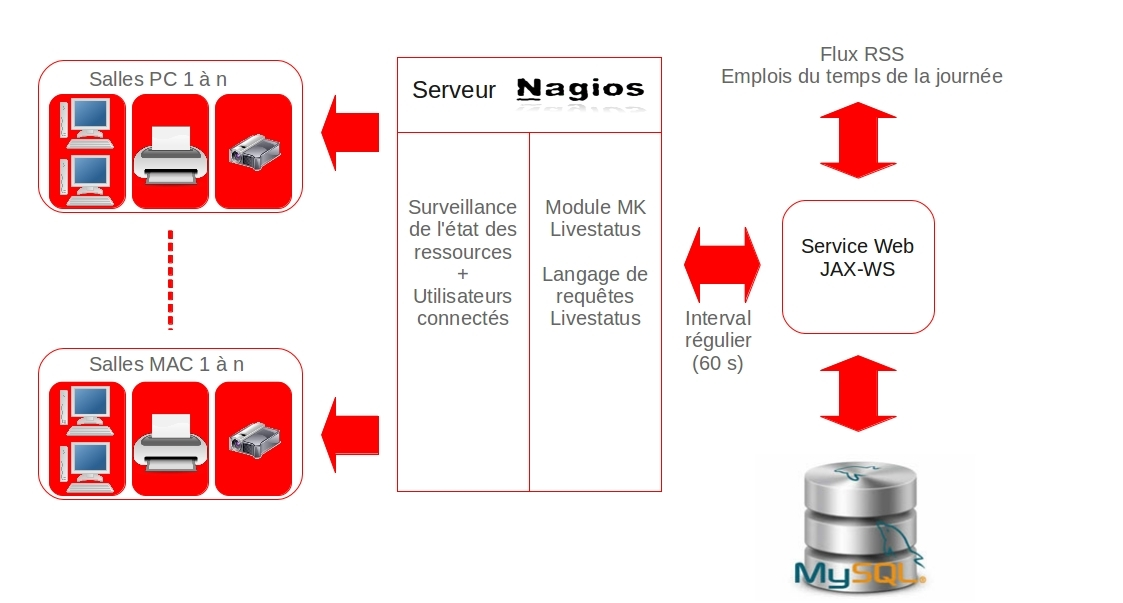
\includegraphics[scale=0.35]{architectureProjetServiceWeb.jpg}
	\caption{Architecture du projet, partie service Web}
	\label{figure:architectureProjetServiceWeb}

\end{figure}

\begin{figure}[!ht]
	\centering
	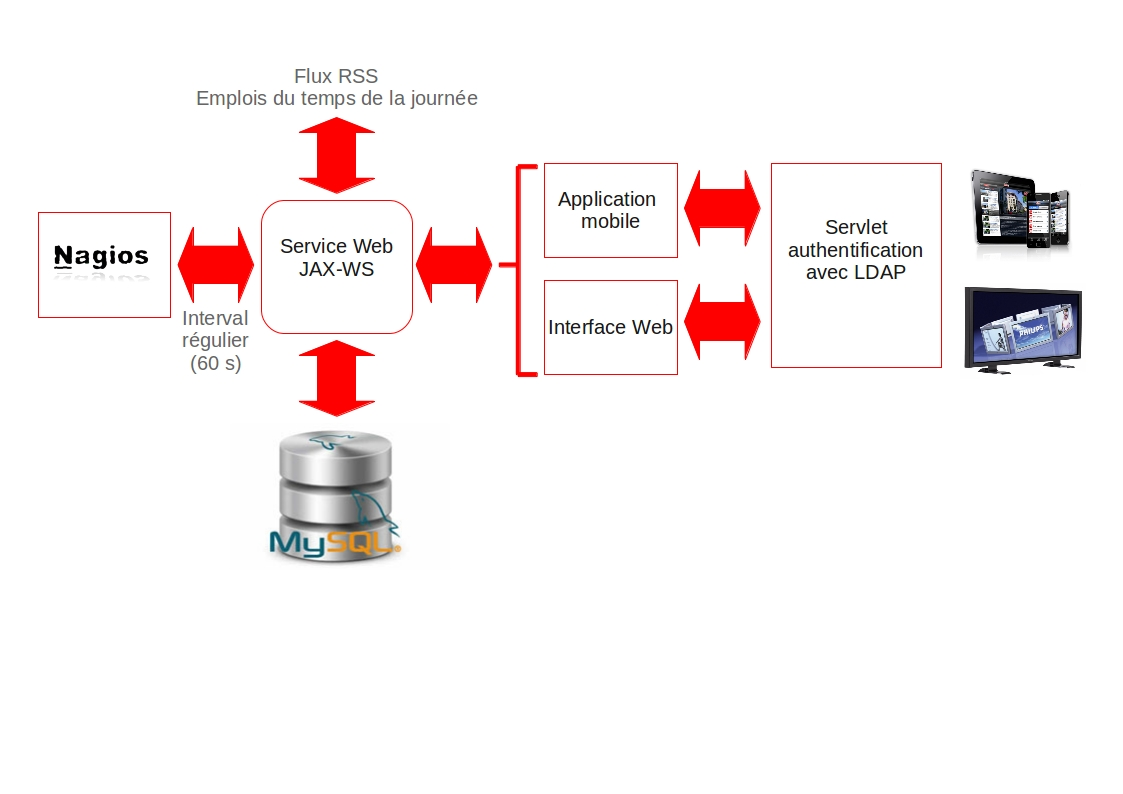
\includegraphics[scale=0.35]{architectureProjetAffichage.jpg}
	\caption{Architecture du projet, partie affichage}
	\label{figure:architectureProjetAffichage}

\end{figure}

Basiquement Nagios sert \`a surveiller les ressources auxquelles il lui est permis d'acc\'eder.
De ce fait, il doit garder des traces des informations qu'il r\'ecup\`ere.
Ces informations sont stock\'ees dans un fichier.
Cependant un plugin a \'et\'e d\'evelopp\'e, \textit{MK Livestatus}, et permet, \`a l'aide d'un langage de requ\^etes qui lui est propre, de r\'ecup\'erer les informations de ce fichier.



\subsection{Nagios}
\label{section:nagios}

\subsection{La notion de service Web}
\label{section:serviceWeb}

\subsection{L'API JAX-WS}

\subsection{L'IDE NetBeans}

\subsection{Le serveur Web Glassfish}

\subsection{Le SGBD MySQL}

\subsection{Data Access Object}

\subsection{Le format JSON}

\section{Communication avec Nagios}

\subsection{Le plugin MK Livestatus}

\subsection{Requ\^etes pour Nagios}

\subsection{R\'ecup\'eration des informations}

\section{Gestion de la base de donn\'ees}

\subsection{Structure de la base de donn\'ees}

\subsection{Explications}

\subsection{G\'en\'eration de la configuration Nagios \`a partir de la base de donn\'ees}

\section{Le service Web}

\subsection{Mise en place}

\subsection{Le cycle principal}

\subsection{Les fonctionnalit\'es publiques}

\subsection{Les fonctionnalit\'es priv\'ees}

\subsection{Le retour des informations}

\subsection{S\'ecurisation du service Web}

\section{Gestion de l'emploi du temps}

\subsection{Les flux RSS de l'universit\'e}

\subsection{Correspondance des salles}

\section{Tests du service Web}

\subsection{Mise en place d'un client}

\subsection{Consommation les m\'ethodes}

\section{Am\'eliorations possibles}

\section{Probl\`emes rencontr\'es}


\clearpage
